\documentclass[11pt]{article}

\usepackage[colorlinks=true]{hyperref}

% This is a toggle for whether the solutions should be included in output of this document
\newif\ifSolutions
%\Solutionsfalse  % this is used to exclude the solutions
\Solutionstrue  % this is used to include the solutions


\usepackage[left=0.8in, right=0.8in, top=0.7in, bottom=1in, includefoot]{geometry}
\usepackage{fancyhdr}
\usepackage{array}
\usepackage{multicol}
\setlength{\parindent}{0mm}
\setlength{\parskip}{5pt}
\usepackage{sectsty}
\allsectionsfont{\sffamily}
\setlength{\headheight}{2cm}
\usepackage{amsmath,amssymb,bm}
\usepackage{booktabs}
\usepackage{graphicx}
\usepackage{color}
\usepackage{cancel}
\usepackage{comment}
\usepackage{hyperref}
\usepackage{subfig}
\usepackage{multirow}
\usepackage{placeins}

% Global definitions
%
% boldface letters
%
%\newcommand{\boldface}[1]{\mathbf{#1}}   % upright
\newcommand{\boldface}[1]{\boldsymbol{#1}}  % italic (slanted)
%
\newcommand{\bfa}{\boldface{a}}
\newcommand{\bfb}{\boldface{b}}
\newcommand{\bfc}{\boldface{c}}
\newcommand{\bfd}{\boldface{d}}
\newcommand{\bfe}{\boldface{e}}
\newcommand{\bff}{\boldface{f}}
\newcommand{\bfg}{\boldface{g}}
\newcommand{\bfh}{\boldface{h}}
\newcommand{\bfi}{\boldface{i}}
\newcommand{\bfj}{\boldface{j}}
\newcommand{\bfk}{\boldface{k}}
\newcommand{\bfl}{\boldface{l}}
\newcommand{\bfm}{\boldface{m}}
\newcommand{\bfn}{\boldface{n}}
\newcommand{\bfo}{\boldface{o}}
\newcommand{\bfp}{\boldface{p}}
\newcommand{\bfq}{\boldface{q}}
\newcommand{\bfr}{\boldface{r}}
\newcommand{\bfs}{\boldface{s}}
\newcommand{\bft}{\boldface{t}}
\newcommand{\bfu}{\boldface{u}}
\newcommand{\bfv}{\boldface{v}}
\newcommand{\bfw}{\boldface{w}}
\newcommand{\bfx}{\boldface{x}}
\newcommand{\bfy}{\boldface{y}}
\newcommand{\bfz}{\boldface{z}}
%
\newcommand{\bfA}{\boldface{A}}
\newcommand{\bfB}{\boldface{B}}
\newcommand{\bfC}{\boldface{C}}
\newcommand{\bfD}{\boldface{D}}
\newcommand{\bfE}{\boldface{E}}
\newcommand{\bfF}{\boldface{F}}
\newcommand{\bfG}{\boldface{G}}
\newcommand{\bfH}{\boldface{H}}
\newcommand{\bfI}{\boldface{I}}
\newcommand{\bfJ}{\boldface{J}}
\newcommand{\bfK}{\boldface{K}}
\newcommand{\bfL}{\boldface{L}}
\newcommand{\bfM}{\boldface{M}}
\newcommand{\bfN}{\boldface{N}}
\newcommand{\bfO}{\boldface{O}}
\newcommand{\bfP}{\boldface{P}}
\newcommand{\bfQ}{\boldface{Q}}
\newcommand{\bfR}{\boldface{R}}
\newcommand{\bfS}{\boldface{S}}
\newcommand{\bfT}{\boldface{T}}
\newcommand{\bfU}{\boldface{U}}
\newcommand{\bfV}{\boldface{V}}
\newcommand{\bfW}{\boldface{W}}
\newcommand{\bfX}{\boldface{X}}
\newcommand{\bfY}{\boldface{Y}}
\newcommand{\bfZ}{\boldface{Z}}

\newcommand{\bfFe}{\boldface{F}_{\text{e}}}
\newcommand{\bfFp}{\boldface{F}_{\text{p}}}
\newcommand{\bfepse}{\pmb{\varepsilon}_{\text{e}}}
\newcommand{\bfepsp}{\pmb{\varepsilon}_{\text{p}}}
\newcommand{\bfeps}{\pmb{\varepsilon}}

%
% boldface greek symbols
%
\newcommand{\bfalpha}{\boldsymbol{\alpha}}
\newcommand{\bfbeta}{\boldsymbol{\beta}}
\newcommand{\bfgamma}{\boldsymbol{\gamma}}
\newcommand{\bfdelta}{\boldsymbol{\delta}}
\newcommand{\bfepsilon}{\pmb{\varepsilon}}
\newcommand{\bfzeta}{\boldsymbol{\zeta}}
\newcommand{\bfeta}{\boldsymbol{\eta}}
\newcommand{\bftheta}{\boldsymbol{\theta}}
\newcommand{\bfkappa}{\boldsymbol{\kappa}}
\newcommand{\bflambda}{\boldsymbol{\lambda}}
\newcommand{\bfrho}{\boldsymbol{\rho}}
\newcommand{\bfmu}{\boldsymbol{\mu}}
\newcommand{\bfnu}{\boldsymbol{\nu}}
\newcommand{\bfpi}{\boldsymbol{\pi}}
\newcommand{\bfxi}{\boldsymbol{\xi}}
\newcommand{\bfsigma}{\boldsymbol{\sigma}}
\newcommand{\bftau}{\boldsymbol{\tau}}
\newcommand{\bfphi}{\boldsymbol{\phi}}
\newcommand{\bfvarphi}{\boldsymbol{\varphi}}
\newcommand{\bfchi}{\boldsymbol{\chi}}
\newcommand{\bfomega}{\boldsymbol{\omega}}
\newcommand{\bfnull}{\boldsymbol{0}}
%
\newcommand{\bfGamma}{\boldsymbol{\Gamma}}
\newcommand{\bfDelta}{\boldsymbol{\Delta}}
\newcommand{\bfTheta}{\boldsymbol{\Theta}}
\newcommand{\bfLambda}{\boldsymbol{\Lambda}}
\newcommand{\bfPi}{\boldsymbol{\Pi}}
\newcommand{\bfXi}{\boldsymbol{\Xi}}
\newcommand{\bfSigma}{\boldsymbol{\Sigma}}
\newcommand{\bfPhi}{\boldsymbol{\Phi}}
\newcommand{\bfChi}{\boldsymbol{\Chi}}
\newcommand{\bfOmega}{\boldsymbol{\Omega}}
\newcommand{\bfnabla}{\boldsymbol{\nabla}}
\newcommand{\laplace}{\boldsymbol{\Delta}}
%
% caligraphic letters
%
\newcommand{\calA}{\mathcal{A}}
\newcommand{\calB}{\mathcal{B}}
\newcommand{\calC}{\mathcal{C}}
\newcommand{\calD}{\mathcal{D}}
\newcommand{\calE}{\mathcal{E}}
\newcommand{\calF}{\mathcal{F}}
\newcommand{\calG}{\mathcal{G}}
\newcommand{\calH}{\mathcal{H}}
\newcommand{\calI}{\mathcal{I}}
\newcommand{\calJ}{\mathcal{J}}
\newcommand{\calK}{\mathcal{K}}
\newcommand{\calL}{\mathcal{L}}
\newcommand{\calM}{\mathcal{M}}
\newcommand{\calN}{\mathcal{N}}
\newcommand{\calO}{\mathcal{O}}
\newcommand{\calP}{\mathcal{P}}
\newcommand{\calQ}{\mathcal{Q}}
\newcommand{\calR}{\mathbb{R}}
\newcommand{\calS}{\mathcal{S}}
\newcommand{\calT}{\mathcal{T}}
\newcommand{\calU}{\mathcal{U}}
\newcommand{\calV}{\mathcal{V}}
\newcommand{\calW}{\mathcal{W}}
\newcommand{\calX}{\mathcal{X}}
\newcommand{\calY}{\mathcal{Y}}
\newcommand{\calZ}{\mathcal{Z}}
% .. define more if needed
%
% double stroke
%
\newcommand{\dsA}{\mathbb{A}}
\newcommand{\dsB}{\mathbb{B}}
\newcommand{\dsC}{\mathbb{C}}
\newcommand{\dsD}{\mathbb{D}}
\newcommand{\dsE}{\mathbb{E}}
\newcommand{\dsF}{\mathbb{F}}
\newcommand{\dsG}{\mathbb{G}}
\newcommand{\dsH}{\mathbb{H}}
\newcommand{\dsI}{\mathbb{I}}
\newcommand{\dsJ}{\mathbb{J}}
\newcommand{\dsK}{\mathbb{K}}
\newcommand{\dsL}{\mathbb{L}}
\newcommand{\dsM}{\mathbb{M}}
\newcommand{\dsN}{\mathbb{N}}
\newcommand{\dsO}{\mathbb{O}}
\newcommand{\dsP}{\mathbb{P}}
\newcommand{\dsQ}{\mathbb{Q}}
\newcommand{\dsR}{\mathbb{R}}
\newcommand{\dsS}{\mathbb{S}}
\newcommand{\dsT}{\mathbb{T}}
\newcommand{\dsU}{\mathbb{U}}
\newcommand{\dsV}{\mathbb{V}}
\newcommand{\dsW}{\mathbb{W}}
\newcommand{\dsX}{\mathbb{X}}
\newcommand{\dsY}{\mathbb{Y}}
\newcommand{\dsZ}{\mathbb{Z}}



\newcommand{\vect}[1]{\mathbf{#1}}
\newcommand{\grvect}[1]{\mbox{\boldmath{$#1$}}}
\newcommand{\perm}{\mbox{{\Huge $\epsilon$}}}
\newcommand{\transvect}[1]{\vect{#1}^{\mbox{\footnotesize T}}}
\newcommand{\invvect}[1]{\vect{#1}^{\mbox{\footnotesize -1}}}
\newcommand{\partderiv}[2]{\frac{\partial #1}{\partial #2}}
\newcommand{\partderivv}[2]{\frac{\partial^2 #1}{\partial #2^2}}
\newcommand{\totalderiv}[2]{\frac{d #1}{d #2}}

\newcommand{\mg}[1]{{\boldsymbol{#1}}}
\newcommand{\mf}[1]{{\mathfrak{#1}}}
\newcommand{\mfb}[1]{{\boldsymbol{\mathfrak{#1}}}}
\newcommand{\ms}[1]{{\mathscr{#1}}}
\newcommand{\mb}[1]{{\mathbf{#1}}}
\newcommand{\mbb}[1]{{\mathbb{#1}}}
\newcommand{\mbbu}[1]{{\underline{\mathbb{#1}}}\vphantom{#1}}
\newcommand{\mbu}[1]{{\underline{\mathbf{#1}}}\vphantom{#1}}
\newcommand{\mgu}[1]{{\underline{\boldsymbol{#1}}}\vphantom{#1}}
\newcommand{\mr}[1]{{\mathrm{#1}}}
\newcommand{\msf}[1]{{\mathsf{#1}}}
\newcommand{\msfb}[1]{{\boldsymbol{\mathsf{#1}}}}

\newcommand{\dotprod}{\stackrel{\scriptscriptstyle \bullet}{}}
\newcommand{\half}{\frac{1}{2}}
\newcommand{\T}{^{\mathsf{T}}} % x^{T}
\newcommand{\mT}{^{\mathsf{-T}}} % x^{-T}
\newcommand{\wass}{\mathsf{wass}}
\newcommand{\eff}{\mathsf{eff}}
\newcommand{\me}{^{\mathrm{-1}}} % x^{-1}
\newcommand{\Rset}{\ensuremath{\mathbb{R}}}
\newcommand{\Kset}{\ensuremath{K}}
\newcommand{\bul}{$\bullet\;$}
%\newcommand{\red}{\mathrm{red}}
\newcommand{\Fe}{\mathbf{F}_\mathbf{e}}
\newcommand{\Fp}{\mathbf{F}_\mathbf{p}}
\def\rel{{\mathrm{rel}}}

%\newcommand{\D}{\displaystyle}
\newcommand{\abs}{\rule[-1cm]{0cm}{1cm}}
\newcommand{\babs}{\rule[-1cm]{0cm}{2cm}}

\newlength{\boxwidth}
\setlength{\boxwidth}{\textwidth}
\addtolength{\boxwidth}{-1cm}

\newcommand\pl{\partial}
\def\dd{\;\!\mathrm{d}}
\def\DD{\;\!\mathrm{D}}
\def\Lin{\R^{d\times d}} 
\def\R{I\!R}
\def\AM{{\mathrm{AM}}}

\def\btheorem{\begin{theorem}}
\def\etheorem{\end{theorem}}
\def\blemma{\begin{lemma}}
\def\elemma{\end{lemma}}
\def\bproposition{\begin{proposition}}
\def\eproposition{\end{proposition}}
\def\bcorollary{\begin{corollary}}
\def\ecorollary{\end{corollary}}
\def\bdefinition{\begin{definition}}
\def\edefinition{\end{definition}}
\def\bexample{\begin{example}}
\def\eexample{\end{example}}
\def\bremark{\begin{remark}}
\def\eremark{\end{remark}}
\def\bproblem#1{\medskip \noindent {\bf #1}\sl \\ }
\def\eproblem{\rm \medskip}
\newcommand{\bma}{ \left( \ba}
\newcommand{\ema}{ \ea \right)}
\newcommand{\set}[2]{\big\{\: #1 \: \big| \: #2 \:\big\} }
\def\cD{\mathcal{D}}
\def\cL{\mathcal{L}}
\def\cG{\mathcal{G}}
\def\cI{\mathcal{I}}
\def\cJ{\mathcal{J}}
\def\ccA{\mathcal{A}}
\def\rmD{\mathrm{D}}
\def\bbQ{\mathbb{Q}}
\def\bbA{\fg{A\!\!\!A}}
\def\fg{\boldsymbol}
\def\mdot{\fg{:}}
\def\vdot{\fg{\cdot}}
\newcommand{\el}{\mathsf{el}}
\def\id{{\bfI}}
\def\eqldef{{\:{\stackrel{\mathrm{def}}{=}}\:}}
\newcommand{\eps}{\varepsilon}
\def\ol{\overline}
\def\wt{\widetilde}
\def\wh{\widehat}
\def\ds{\displaystyle}
\def\ts{\textstyle}
\def\mtr{^\mathrm{-T}}
\def\inh{^\mathrm{inh}}
\DeclareMathOperator{\divv}{div}
\DeclareMathOperator{\grad}{grad}
\DeclareMathOperator{\tr}{tr}
\DeclareMathOperator{\curl}{curl}
\DeclareMathOperator{\Curl}{Curl}
%\DeclareMathOperator{\T}{T}
\DeclareMathOperator{\argmin}{{arg\,min}}
\DeclareMathOperator{\diag}{diag}
\DeclareMathOperator{\trace}{tr}
\DeclareMathOperator{\sign}{sign}
\DeclareMathOperator{\dev}{dev}
\DeclareMathOperator{\cof}{cof}
\DeclareMathOperator{\sym}{sym}
\DeclareMathOperator{\skews}{skw}
\def\Felast{\bfF_\mathbf{\!e}}
\def\Fplast{\bfF_\mathbf{\!p}}
\def\Cplast{\bfC_\mathbf{\!p}}
\def\epselast{\bfeps_\mathbf{\!e}}
\def\epsplast{\bfeps_\mathbf{\!p}}
\def\GLin{\mbox{{\sf GL}$(d)$}}  %{\R^{d\times d}_*}% invertible matrices
\def\Lin{\R^{d\times d}}        % all d times d matrices
\def\reff#1{(\ref{#1})}
\def\red{{\mathrm{red}}}
\def\rep{{\mathrm{rep}}}
\def\cond{{\mathrm{cond}}}
\newcommand{\kopfcolor}{\color{red}}
\newcommand{\er}{\hspace*{4cm}}
\newcommand{\n}{{\rm n}}
\newcommand{\nn}{{\rm n+1}}
\newcommand{\PsiS}{\Psi_\mathrm{S}}
\newcommand{\PsiV}{\Psi_\mathrm{V}}
\newcommand{\PsiI}{\Psi_\mathrm{I}}
\newcommand{\cA}{c_\mathrm{A}}
\newcommand{\cM}{c_\mathrm{M}}

\newcommand{\calAe}{\underset{e=1}{\overset{n_e}{\mathcal{A}}}}
\newcommand{\Grad}{\text{Grad}}
\newcommand{\tcr}{\tau_{\text{crit}}}
\newcommand{\be}{\begin{equation}\nonumber}
\newcommand{\ee}{\end{equation}}
\newcommand{\beq}{\begin{eqnarray}}
\newcommand{\eeq}{\end{eqnarray}}
\newcommand{\bem}{\begin{multline}}
\newcommand{\eem}{\end{multline}}
\newcommand{\ba}{\begin{align}}
\newcommand{\ea}{\end{align}}
\newcommand{\bfzero}{{\fg0}}

\renewcommand{\figurename}{Figure}
\renewcommand{\tablename}{Table}

\newcommand{\fp}[2]{\frac{\partial #1}{\partial #2} }
\newcommand{\LR}{{\qquad \Leftrightarrow \qquad }}
\newcounter{problem}
\newcounter{points}
\newcounter{stretchPoints}

\newcommand{\head}[3]{

\begin{center}
\section*{Homework Set \##1 \ifSolutions Solutions \fi}
assigned: #2\\
due: #3, 11:00 pm\\
in your repo at /cs/cs181j/2015/fall/students/your\_user\_name/cs181j \\
\end{center}
\hrule
\vskip 0.1cm
}

\newcommand{\prob}[1]{\par\vskip 0.5cm \stepcounter{problem}\subsubsection*{Problem \arabic{problem} \ \small (#1 points).}\addtocounter{points}{#1}}
\newcommand{\total}{
\begin{flushright}
\small\par\vskip 0.3cm \textit{total: \arabic{points} points ({\color{blue}+\arabic{stretchPoints} stretch points})}
\end{flushright}
}

\newcommand{\eprob}[2]{\par\vskip 0.5cm \stepcounter{problem}\subsubsection*{Problem \arabic{problem}: #2 \ \small (#1 points).}\addtocounter{points}{#1}}

\newcommand{\estretchprob}[3]{\par\vskip 0.5cm \stepcounter{problem}\subsubsection*{Problem \arabic{problem}: #3 \ \small (#1 points ({\color{blue}+#2 stretch points}) ).}\addtocounter{points}{#1}\addtocounter{stretchPoints}{#2}}


%\endinput

\usepackage{afterpage}
\usepackage{enumerate}

\begin{document}
\sffamily
\pagestyle{fancy}
\renewcommand{\headrulewidth}{0.4pt}
\fancyfoot[C]{\sffamily \thepage{}}
\fancyhead[C]{\vskip 0.7cm \sffamily\footnotesize \textbf{cs181j -- High Performance Computing} \hfill \name\\ Fall 2015 \hfill Harvey Mudd College}

% Convenience function used for including a figure
\newcommand\Figure[3]
{
    \begin{figure}[h!]
        \begin{center}
    \includegraphics[width=#3 in]{#1}
    \caption{\label{fig:#1} {#2}}
    \end{center}
    \end{figure}
}

\newcommand\TwoFigure[7]
{
    \begin{figure}[h!]
        \subfloat[#2]{\includegraphics[width=#7 in]{#1}}
    \hfill
        \subfloat[#4]{\includegraphics[width=#7 in]{#3}}
        \caption{\label{fig:#6}#5}
    \end{figure}
}

\newcommand\TwoFigureVertical[7]
{
    \begin{figure}[h!]
        \subfloat[#2]{\includegraphics[width=#7 in]{#1}}

        \subfloat[#4]{\includegraphics[width=#7 in]{#3}}
        \caption{\label{fig:#6}#5}
    \end{figure}
}


\fancyhead[RL]{}

%\newcommand{\name}{I forgot to change my name}


\head{11}{Monday, November 30, 2015}{Friday, December 4, 2015}

On the last assignment, we were just trying to get CPU programs to \emph{run at all} on a GPU without really thinking about getting good performance.  
On this assignment, we'll care about memory access to improve our performance.  

\estretchprob{15}{10}{Cuda Finite Difference Wave Equation}

In this problem, you'll make a finite difference wave equation solver that uses cuda to do the number crunching.  
Now, to be honest, this isn't the \textit{best} algorithm in the world to cuda-ize because it's just so darned cheap, but it's still a good exercise.

The easiest way to use a GPU in a simulation is to do it ``non-invasively'', something like what's described on the slide titled ``Maybe Okayish but Probably Not GPU Molecular Dynamics Example'', where every time you're about to crunch numbers, you ship the data to the GPU, do the computation, and ship it back. 
It is easy to incorporate cuda into simulations in this non-invasive fashion, but it can have serious performance penalties because of the cost of shipping data back and forth.  

The better way to incorporate cuda is to leave the data on the GPU as much as you can, and only pull over copies of it to the CPU when you need to do things such as write output files.  
However, this often requires an architectural change to your simulation code (or you design for it from the beginning) because now data can either be living on the CPU or the GPU.  

\textbf{Note:} I have provided some starter code in \texttt{.cu} files, which are being compiled with nvidia's compiler and I've removed all non-compatible c++ from the \texttt{Cuda1DFDWave*} files so that you don't have to have three separate files for these problems; you can write your cuda kernels and such directly in the files.

\textbf{Note:} Don't use shared memory on this problem unless you like pain, sadness, and doing more work for no credit whatsoever.

\textbf{Note:} Remember to disable file writing when comparing speeds!

\begin{enumerate}[a)]
\item Implement a version of the wave equation solver that uses cuda ``non-invasively'' (i.e. that ships information back and forth each timestep).  
Include a couple of plots (boo!) or a link to a movie (yay!) that show a waveform moving through the domain.  
More or less, how much faster is the ``non-invasive'' cuda version than the threaded CPU version you made?

\ifSolutions
\textbf{Solution:}

\href{https://www.youtube.com/watch?v=dQw4w9WgXcQ}{Here} is the link to my fantabulous movie.

\fi

\item Implement a version of the wave equation solver that uses cuda ``invasively'' (i.e. that leaves the data on the GPU except when it needs to write output files). 
Include a couple of plots (or a link to a movie) that show a waveform moving through the domain.  
More or less, how much faster is the ``invasive'' cuda version than the threaded CPU version?

\ifSolutions
\textbf{Solution:}

\href{https://www.youtube.com/watch?v=dQw4w9WgXcQ}{Here} is the link to my fantabulous movie.

\fi

\item For 10 stretch points, implement an ``invasive'' version of the wave equation solver purely using \emph{no cuda} kernels, just using \href{http://docs.nvidia.com/cuda/thrust/#axzz3KKFtexoj}{thrust}.  
See thrust \href{http://docs.nvidia.com/cuda/thrust/#transformations}{transformations}, which may be helpful.  How does the thrust version performance compare to your cuda ``invasive'' version?
\end{enumerate}

\ifSolutions
\textbf{Solution:}

\fi

\vfill

%\newpage







\eprob{35}{Many Matrix Multiplications}

Soon, we'll make a single matrix multiplication faster by using shared memory.  
However, to be honest, the answer to doing a single fast matrix multiplication is not to use the neat version that you write, but to use cublas, nvidia's library for matrix stuff.
This is kind of discouraging because it's no fun when the answer is ``use a library because it's smarter than you.''

However, consider the case of doing not just one matrix multiplication, but many.  
Perhaps you're doing 10 large matrix multiplications, or 100,000 small matrix multiplications.  
Using cublas to do 100,000 small matrix mutliplications individually is a bad idea, so we're going to write a program that that multiplies not just one matrix but some number of pairs of matrices of equal size.  
Your program has to work well multiplying, for example, perhaps 100000 pairs of 5x5 matrices or 1 pair of 2000x2000 matrices, or anything between.  
You'll first write a threaded CPU version, after which you'll analyze and then write a couple flavors of GPU versions.

Remember, we're forgetting about using shared memory and we're just considering global memory access patterns.

\begin{enumerate}[a)]
\item Answer these next few questions before you do any googling on the subject.  Consider the following naive serial version of the ``many matrix multiplications'' algorithm:
\begin{verbatim}
for matrixIndex = 0 to numberOfMatricesToMultiply
  for each row in the resultant matrix
    for each column in the resultant matrix
      sum = 0
      for dummy = 0 to matrixSize
        sum += leftMatrices[matrixIndex](row, dummy) *
               rightMatrices[matrixIndex](dummy, col)
      resultMatrices[matrixIndex](row, col) = sum
\end{verbatim}

If you were threading this with \texttt{openmp} and were constrained to only be able to put in a single line with \texttt{pragma omp parallel for}, before which for loop would you put it?  
Would your proposed position be effective for the case of multiplying many small matrices, the case of multiplying a couple large matrices, or all cases?

\textbf{Note:} When describing where you'd put the \texttt{pragma}, be very specific; say things such as ``the for each column'' loop and don't say ambiguous things like ``inner loops'' or ``outer loops''.

\ifSolutions
\textbf{Solution:}

\fi

\item If you were only allowed to use a single \texttt{pragma omp parallel for} line with nothing more on it, how can you change your loop structure to get effective threading for all cases?

\ifSolutions
\textbf{Solution:}

\fi

\item Read about the openmp \texttt{collapse} clause \href{https://computing.llnl.gov/tutorials/openMP/}{here} (search for collapse) and \href{http://www.openmp.org/mp-documents/OpenMP4.0.0.pdf}{here} (page 55).  
How does it solve this problem?

\ifSolutions
\textbf{Solution:}

\fi

\item Implement an \texttt{openmp} threaded version in the provided code using the \texttt{collapse} clause.
  
You don't have to worry about plotting anything here, it'll get plotted with the other versions later.

\item For the next few parts, we'll analyze and then implement some GPU versions.  
In class, we talked about how you can have two different threading policies: either the next thread handles the next entry in the same matrix, or the same entry in the next matrix.  
You can also have two different memory layouts: either you can have ``serial matrices'' where the matrices are all stored in order (all of the entries of one matrix, then all of the entries in the next matrix, etc.) or you can use ``deep entries'' where entry (0,0) of all matrices are stored together, then entry (0,1) of all matrices, etc.
The four combinations of threading policy and memory layout are shown in figure \ref{fig:ManyMatrixMultiplicationConfigurations}.

Identify whether the memory accesses for the left, right, and result matrices are broadcast, coalesced, or uncoalesced.  
For the left and right accesses, identify whether you expect the access to be cached or uncached.

\ifSolutions
\textbf{Solution:}

\begin{center}
  \begin{tabular}{ | l || c | c | c |}
    \hline
    configuration & left & right & result \\ \hline \hline
    next thread next entry, serial matrices & TODO & TODO & TODO \\ \hline
    next thread next entry, deep entries & TODO & TODO & TODO \\ \hline
    next thread next matrix, serial matrices & TODO & TODO & TODO \\ \hline
    next thread next matrix, deep entries & TODO & TODO & TODO \\ \hline
  \end{tabular}
\end{center}

\fi

%\FloatBarrier

\item Implement the ``next thread next entry, serial matrices'' version.  
This is very close to just naive row-major times row-major multiplication, you just have to figure out how to deal with multiple matrices.

You don't have to worry about plotting anything here, it'll get plotted with the other versions later.

\textbf{Note:} You are welcome to use the following outline for the kernels in this problem, if it's helpful:

\begin{verbatim}
unsigned long entryIndex = ...
while (entryIndex < totalNumberOfEntries) {
  calculate matrixIndex, row, and col this thread is about to handle using
    the entryIndex and the threading policy
  double sum = 0;
  for (unsigned int dummy = 0; dummy < matrixSize; ++dummy) {
    sum += 
      dev_leftMatrices[ calculate index from matrixIndex, row, and dummy using layout] *
      dev_rightMatrices[calculate index from matrixIndex, col, and dummy using layout]
  }
  entryIndex += totalNumberOfThreads
}
\end{verbatim}

\item Implement the ``next thread next matrix, deep entries'' version.

You don't have to worry about plotting anything here, it'll get plotted with the other versions later.

\item Use the provided script to make a plot of the speedups (compared to serial CPU) of the threaded CPU implementation and all the GPU implementations that you made.  
Comment on these results.  
In particular, does the performance qualitatively match your analysis?
\end{enumerate}

{
  \begin{figure}[h!]
    \begin{center}
    \begin{tabular}{c}
    \subfloat[next thread next entry, serial matrices]{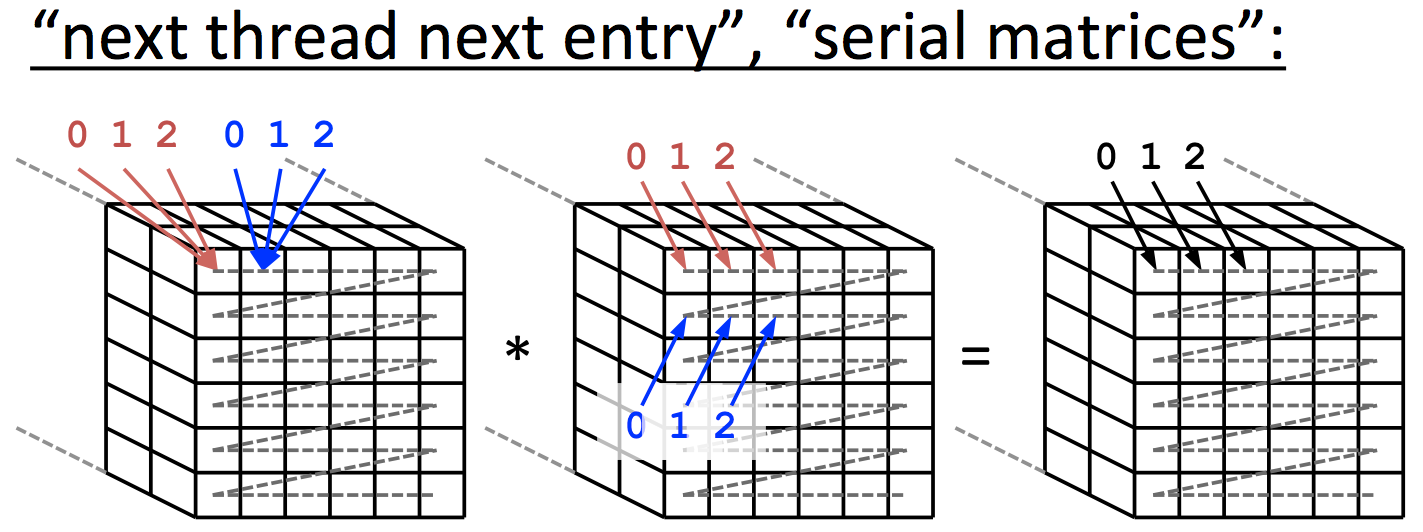
\includegraphics[width=4.25 in]{NextThreadNextEntry_SerialMatrices}} \\
    \subfloat[next thread next entry, deep entries]{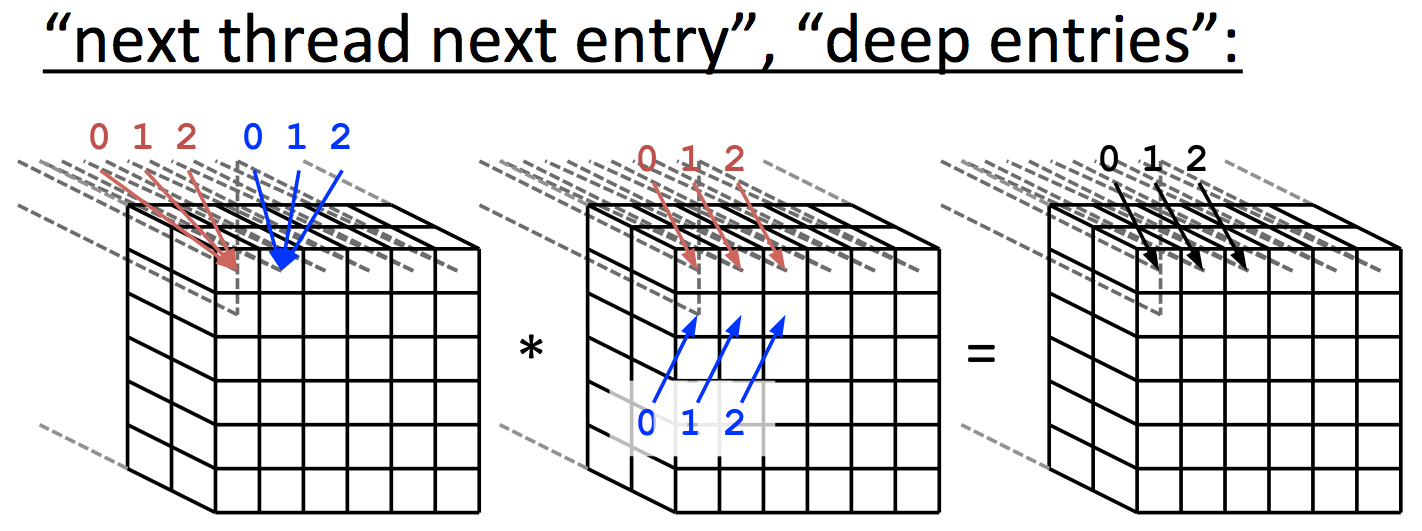
\includegraphics[width=4.25 in]{NextThreadNextEntry_DeepEntries}} \\
    \subfloat[next thread next matrix, serial matrices]{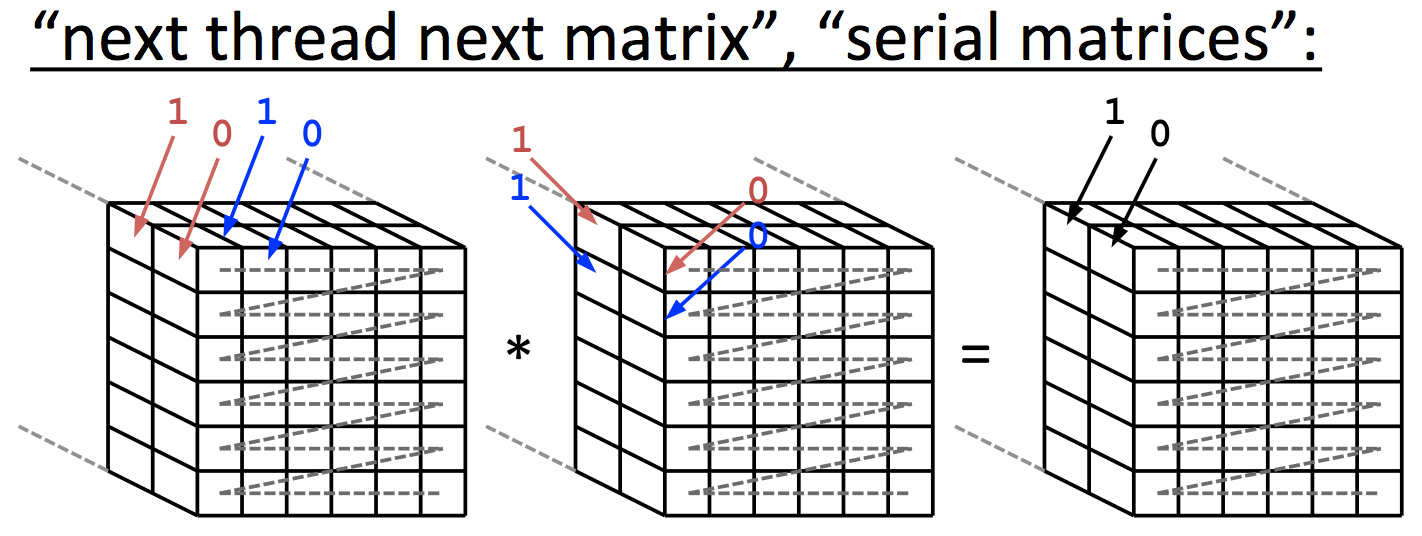
\includegraphics[width=4.25 in]{NextThreadNextMatrix_SerialMatrices}} \\
    \subfloat[next thread next matrix, deep entries]{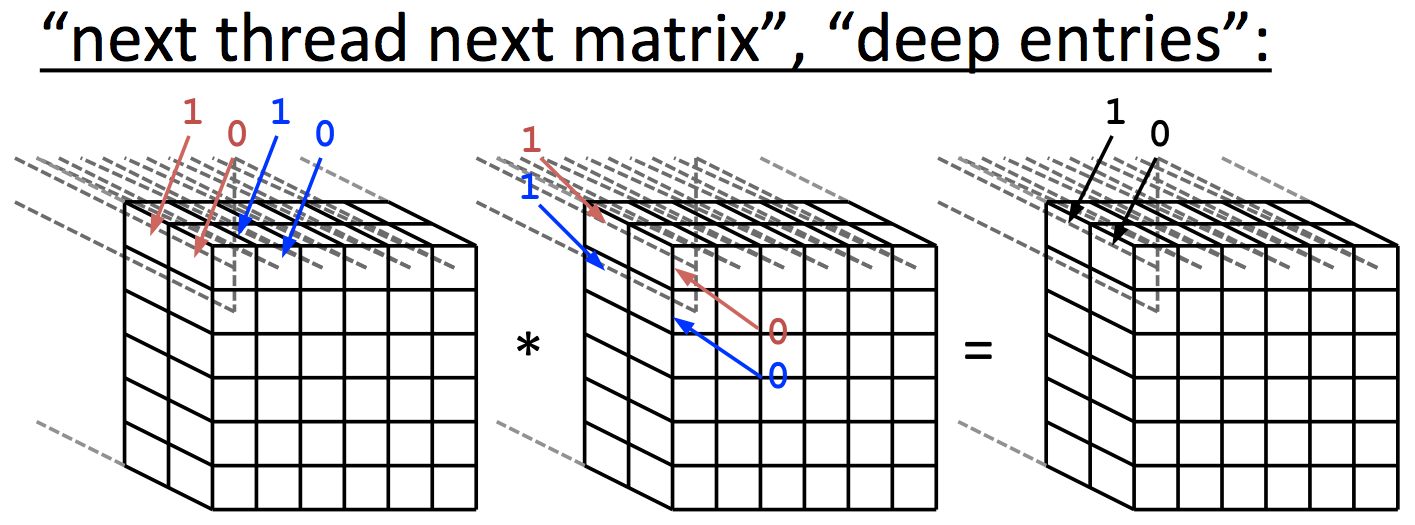
\includegraphics[width=4.25 in]{NextThreadNextMatrix_DeepEntries}} \\
    \end{tabular}
    \end{center}
    \caption{\label{fig:ManyMatrixMultiplicationConfigurations} Configurations for the many matrix multiplication problem.  Red arrow represent reads performed by a thread first, blue arrows represent the next reads, and black arrows represent writes.  Numbers represent thread indices.}
  \end{figure}
}

\ifSolutions
\textbf{Solution:}

{
  \begin{figure}[h!]
    \begin{center}
    \begin{tabular}{c}
    \subfloat{
\includegraphics[width=6.0 in]{figures/ManyMatrixMultiplications_speedup_shuffler}} \\
    \end{tabular}
    \end{center}
    \caption{Speedup of various gpu versions versus input size}
    \label{fig:Problem3}
  \end{figure}
}

\fi

\vfill

%\newpage









\eprob{20}{Single Matrix Multiplication}

Our matrix multiplication version from the last assignment worked fairly well, but there was a fairly significant gap between our performance and that of cublas.  
This is not necessarily unexpected: we don't use shared memory, we aren't using a sophisticated multiplication algorithm, and the NVIDIA people had better know how to use their cards better than we do.  
We'll remedy one of those differences on this problem.

Implement the ``row major storage, tiled multiplication'' technique using shared memory.  
Use a fixed \\ \texttt{numberOfThreadsPerBlock} of 1024 and a fixed \texttt{tileSize} of 32, and implement the following algorithm (illustrated in figure \ref{fig:tiled_blocks_threads}):

\begin{verbatim}
resultTileIndex = blockIndex
while (resultTileIndex < numberOfTiles)
  for dummyTile from 0 to numberOfTilesPerSide
    load leftTiles(resultTileRow, dummyTile) and
      rightTiles(dummyTile, resultTileCol) into shared memory
    resultTiles(resultTileRow, resultTileCol) +=
      leftTileInSharedMemory * rightTileInSharedMemory
  resultTileIndex += numberOfBlocks
\end{verbatim}

Use the provided script to make a plot of the speedup (compared to serial CPU) of your shared memory version and cublas.  
How good is your best version compared to \texttt{cublas}?  
How much did using shared memory improve your implementations?

{
  \begin{figure}[h!]
    \begin{center}
    \begin{tabular}{c}
    \subfloat{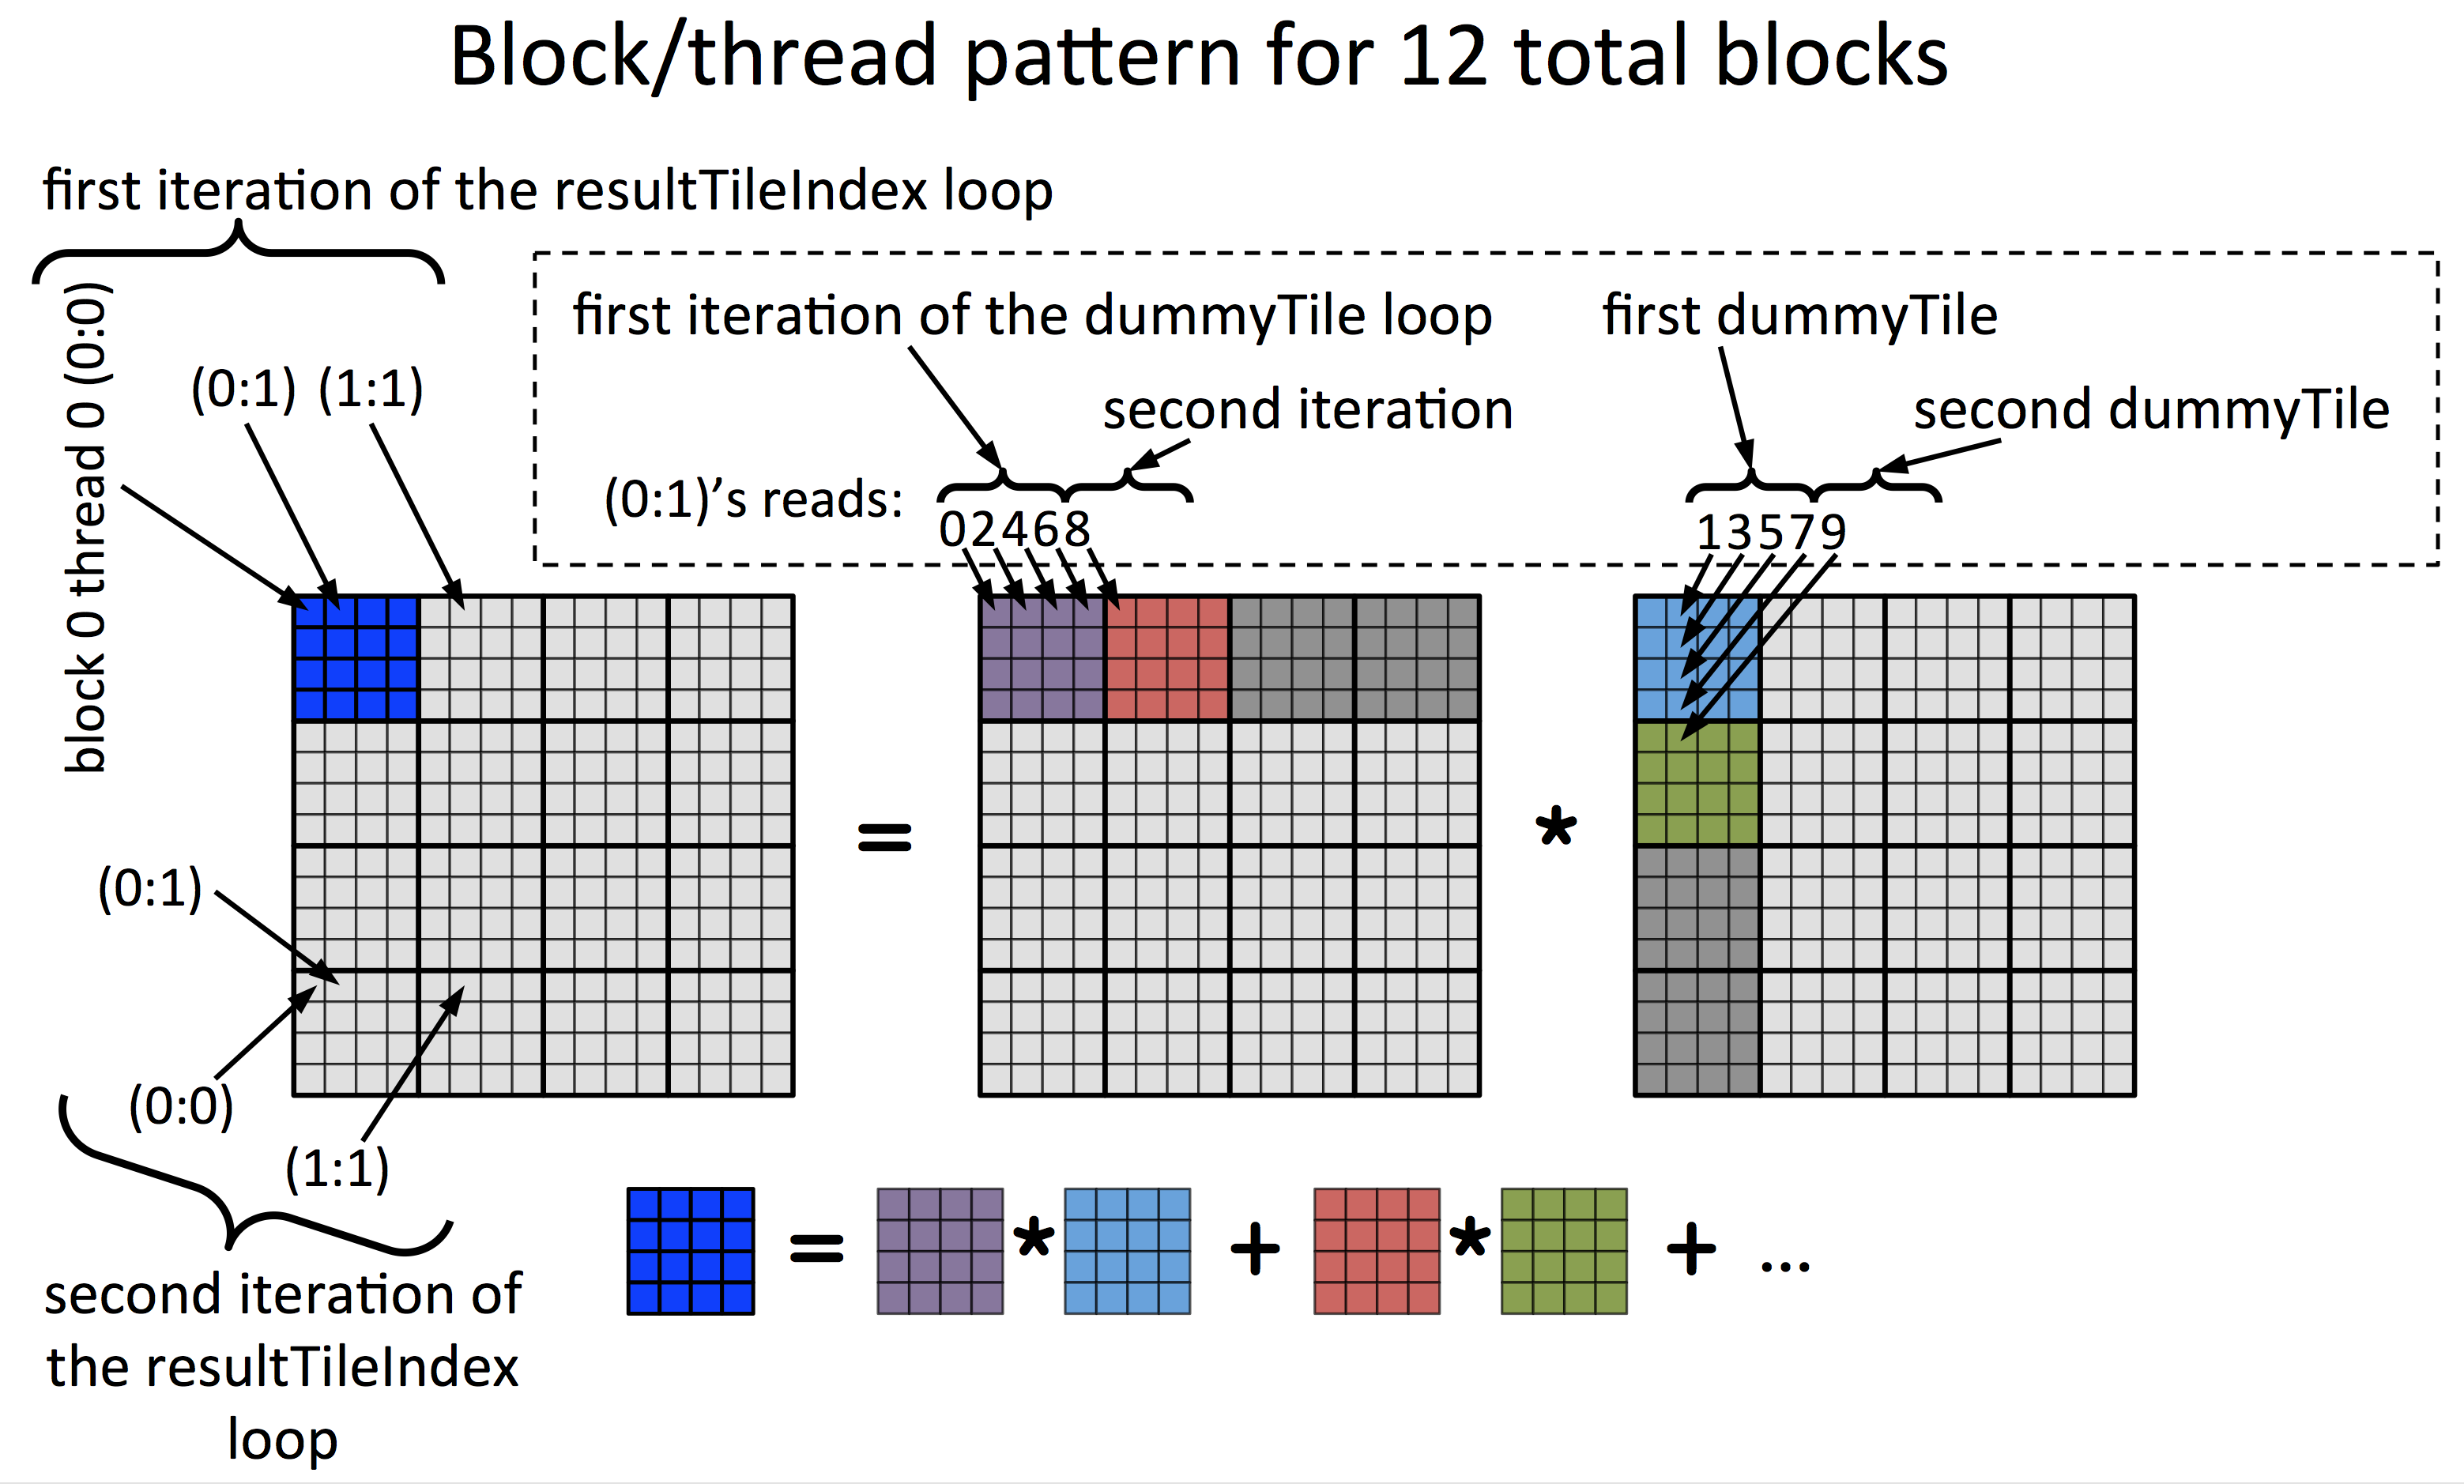
\includegraphics[width=5.0in]{tiled_blocks_threads}} \\
    \end{tabular}
    \end{center}
    \caption{Blocks and threads for tiled multiplication}
    \label{fig:tiled_blocks_threads}
  \end{figure}
}

\ifSolutions
\textbf{Solution}

{
  \begin{figure}[h!]
    \begin{center}
    \begin{tabular}{c}
    \subfloat{
\includegraphics[width=6.0in]{figures/MatrixMultiplication_matrixMultiplication_shuffler}} \\
    \end{tabular}
    \end{center}
    \caption{Performance of matrix multiplication}
    \label{fig:Main4}
  \end{figure}
}

\fi

\vfill

\eprob{15}{Analyzing Memory Accesses}

Suppose that you are tasked with making the following kernel faster, in which consecutive threads get consecutive values of \texttt{atomIndex}:

\begin{verbatim}
...
float x = positions[atomIndex * 3 + 0];
float y = positions[atomIndex * 3 + 1];
float z = positions[atomIndex * 3 + 2];

float force_x = 0;
float force_y = 0;
float force_z = 0;
for (unsigned int neighborNumber = 0; 
     neighborNumber < numberOfNeighborsPerAtom; ++neighborNumber) {
  const unsigned int neighborIndex = 
    neighborLists[atomIndex * numberOfNeighborsPerAtom + neighborIndex];
  const float neighborPosition_x = positions[neighborIndex * 3 + 0];
  const float neighborPosition_y = positions[neighborIndex * 3 + 1];
  const float neighborPosition_z = positions[neighborIndex * 3 + 2];
  ...
}
forces[atomIndex * 3 + 0] = force_x;
forces[atomIndex * 3 + 1] = force_y;
forces[atomIndex * 3 + 2] = force_z;
\end{verbatim}

Let's simply consider memory accesses.
List the memory accesses.  
Will they be coalesced or uncoalesced?
Will they be cached or uncached?
What can you do to make each access better?

\ifSolutions
\textbf{Solution}

\begin{enumerate}
  \item positions[atomIndex * 3 + ...] : this access will be coalarkey and extra-cashy.  You could make it better by giving Jeff a job so that he doesn't have to spend thanksgiving break applying for jobs and not making cool new homework problems.
  \item TODO
\end{enumerate}


\vfill

\newpage

\eprob{10}{Back to the Real World}

Provide short (but sufficient) answers to the following prompts:

\begin{enumerate}[a)]
\item On a GPU, there are many ways to get information to be used by the cuda cores.  
Explain as you would to a ``non-technical'' friend of yours the different places where information can be stored on a GPU (registers, local memory, shared memory, global memory, the texture cache, and the constant cache), and what they're useful for.  
However, don't get too far into shared memory, there's a whole question on that.

\ifSolutions
\textbf{Solution:}

\fi

\item Explain as you would to a ``non-technical'' friend of yours what the difference is between coalesced and uncoalesced global memory access.
  
\ifSolutions
\textbf{Solution:}

\fi

\item Describe a real-life (non-computing-related) example that illustrates the difference between threads in a block using shared memory versus those threads just using global memory.

\ifSolutions
\textbf{Solution:}

\fi

\end{enumerate}

\vfill

\eprob{5}{Feedback}

\begin{enumerate}[a)]
\item How much total time did you spend on this assignment?
\item Of the total time, how much total time did you spend ``flailing'' on little annoying things that are not the main point of the assignment?
\item Of the total time, how much total time did you spend on the stretch problem?
\item Did you have any ``aha'' moments where something clicked?  If so, on what problems or parts?
\item Can you give me any feedback on this assignment?
\end{enumerate}

\vfill

\vskip 1cm
\total

\end{document}

todo: figure out where i could fit in more surprise assignments
